\chapter{Implementation}
\section{Background Theory}
\label{chap:implementation}
When implementing a real time mesh deformation system certain decisions must be made.
Firstly one must decide upon the model to use for the mesh deformation, the more brute-force mass spring system or the algorithmical approach using proper physics.
As previously indicated we are working with a mass spring system for this implementation.

Following the decision of models we need to decide on an integration scheme, how should we model the changes in acceleration, position, and velocity of our vertices?
Many different integration schemes exits, such as explicit Euler integration, Runge Kutta, or Verlet intergration, all with different properties and difficulty of implementation.
The two used in the following implementations will be semi-implicit Euler integration and Verlet integration.
Lastly we need to decide if we go for a kinematic system where we model springs as constraints, 
or a dynamic system where we model the springs as proper springs working with Hooke's law\cite{math_for_games}, both of which are presented within this chapter.

\todo{Talk about how the deformation is done without mentioning springs first. I.e. you apply force to it.}
\todo{Also mention the importance of damping.}
\todo{Motivate that you choose both your "physics model" and your integration scheme}

\think{Firstly one must decide upon the model to use for the mesh deformation itself, i.e. are we algorithmically solving these problems using proper physics, or do we more brute force it through particle simulation. The algorithmic approach using proper physics will usually yield more realistic results, however, they are usually more complicated to implement,
and might not meet the performance requirements of games. The more brute force approaches such as spring-mass spring systems are usually easier to implement,
and gives good enough results.}


%
%\begin{figure}
    %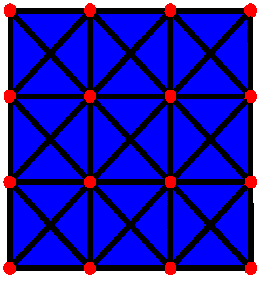
\includegraphics{report/figures/md_fisher_cloth.png}
    %\caption{Caption}
    %\label{fig:my_label}
%\end{figure}
%\todo{Find smaller image}

\subsection{What is Semi-Implicit Euler Integration?}
Semi-Implicit Euler integration is perhaps the integration scheme that is easiest to follow, and comes most natural to programmers when they implement
movement in a realtime system for the first time. It is also a scheme used within a lot of physics engines~\cite{gafferongames_integration}.

In Semi-Implicit Euler integration we keep the total accumulated force, velocity and position of each game object.
Upon each timestepped update of the system we divide all the force that has been applied to an object by the mass of the object to get the acceleration of the object.
Multiplying this acceleration with the timestep yields the change in velocity of the object, which added on the previous velocity becomes the new velocity.
This new velocity is then multiplied with the timestep and added to the position, reflecting the change in position over time.
The code for this can be seen in listing~\ref{code:semi-implicit_euler_integration}.

\begin{figure}
\begin{lstlisting}[label={code:semi-implicit_euler_integration},language=csharp,caption={Semi-Implicit Euler Integration}]
private void SemiImplicitEuler(float dt, GameObject go)
{
    var acceleration = go.force / go.mass;
    go.velocity += acceleration * dt;
    go.position += go.velocity * dt;
}
\end{lstlisting}
\end{figure}

\subsubsection{Advantages \& Disadvantages}
The largest advantage of the semi-implicit Euler integration is its ease of implementation, as well as the generally low computational complexity.
However, it is not entirely stable, meaning that you can get into situations where your numbers start exploding.

\subsection{What is Verlet Integration?}
Rather than storing velocities and positions of each game object like the Euler integration, Verlet integration stores the current and previous positions of each game object.
Per timestep the current velocity is calculated implicitly by subtracting the current position from the previous one.
Changes to the current velocity is also modelled via positional data by integrating the game object's acceleration twice over the timestep.
The new position of a game object following a Verlet integration is then: The current position added with the calculated velocity and the positional change due to acceleration.
Code for this can be seen in listing~\ref{code:verlet_integration}.

\begin{figure}
\begin{lstlisting}[label={code:verlet_integration},language=csharp,caption={Verlet Integration}]
private void Verlet(float dt, GameObject go)
{
    var acceleration = go.force / go.mass;
    var curr = go.pos + (go.pos - go.prevPos) + acceleration * dt * dt;
    go.prevPos = go.pos;
    go.pos = curr;
}
\end{lstlisting}
\end{figure}

\subsubsection{Advantages \& Disadvantages}
Just like semi-implicit Euler integration this integration model is relatively easy to implement, and relatively fast.
Due to the velocity being calculated based on the positions, it is very hard to end up in a situation where the velocities and positions come out of sync,
meaning that the model is quite stable.
I would however argue that while it is easy to implement it is not as easy to understand as the Semi-Implicit Euler integration, at least upon first contact with the model.
I needed a proper intuitive explanation from Mosegaard\cite{mosegaards_clothing_simulation} before I understood what was really going on.
Additionally, Verlet integration, at least with this implementation requires a fixed time step, otherwise the velocity calculation won't be correct~\cite{alan_wake_mass_spring}.

\subsection{Kinematic or Dynamic approach?}
When working with mesh deformation one needs to decide upon a kinematic or a dynamic approach for controlling the springs.

Within a kinematic approach the springs between the vertices are thought of as constraints that you need to solve for.
Essentially this means that if two points are too far apart from each other, you move them a bit closer together, potentially over several iterations to ensure that you are not creating
new inconsistencies in the model.
The kinematic approach is the easiest to implement of the two and can never explode, however, the extra iterations needed to solve the constraints can have performance implications.

The dynamic approach on the other hand models the springs as actual springs that correct themselves through forces according to the laws of physics, such as Hooke's Law.
This approach is much harder to implement, and can lead to situations where the model spirals out of control (i.e. explodes).
Additionally, while implementing soft springs in with this approach is not that difficult, harder springs require more complicated integration schemes\cite{math_for_games}.

While both of these approaches imply different terminology for the connections/springs within a system I will refer to the connections between vertices as springs for the rest of the article, as the name of the model is "mass spring system".

\section{Implementation}
Once all the decisions of deformation model, integration scheme and kinematic/dynamic approach has been made it is possible to start implementation of mesh deformation.

\subsection{Dynamic Approach - Ball Deformation}
\todo{Add video}
Jasper Flick\cite{catlike_mesh_deformation} shows an implementation where the springs are implied based on the original position of each vertex and their new position.
The implementation takes a dynamic approach to deformation and follows a semi-implicit Euler integration scheme.
In this implementation we keep a copy of the initial vertex positions, as well as a collection of the modified vertices.
Additionally, we keep a collection of the velocity of each vertex, which we update each time force is added to a vertex.
The springs come into play when updating the positions of all the vertices based on their velocities.
Each spring within this system is the vector between the initial positions of the vertices in the mesh and their current positions, as seen in figure \ref{fig:catlike_mesh_deformation_springs}.
Upon update of the vertices the force of a spring is applied to the velocity of a vertex in the direction of the spring, moving the vertex back towards its initial position.
The code for this can be seen in listing~\ref{code:catlike_mesh_deformation_update}.

\todo{Write about how force is added}

\begin{figure}
\centering
    \scalebox{0.5}{
    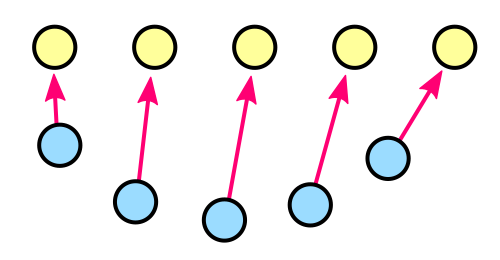
\includegraphics[width=\textwidth]{report/figures/catlike_mesh_deformation_springs.png}
    }
    \caption{Modified vertices(yellow) are pulled towards their original position(blue) by the springs (pink)\cite{catlike_mesh_deformation}}
    \label{fig:catlike_mesh_deformation_springs}
\end{figure}

\begin{figure}
\begin{lstlisting}[label={code:catlike_mesh_deformation_update},language=csharp,caption={Catlike coding mesh deformation vertex update}]
private void UpdateVertex(int i)
{
    Vector3 velocity = mVertexVelocities[i];
    Vector3 spring = mDisplacedVertices[i] - mOriginalVertices[i];
    spring *= UniformScale;
    velocity -= spring * SpringForce * Time.deltaTime;
    velocity *= 1f - Damping * Time.deltaTime;
    mVertexVelocities[i] = velocity;
    mDisplacedVertices[i] += velocity * (Time.deltaTime / UniformScale);
}
\end{lstlisting}
\end{figure}

\subsubsection{Usage}
As seen in the video, although simple, the implementation provides quite a lot of flexibility, toying with the different variables
can lead to some interesting visual effects.
For example, applying negative force to the sphere can be used to create a visual effect similar to that of a star being swallowed by a black hole.
Applying outward force from the inside of the model can create a relatively convincing effect of something moving around inside the object.
Giving the sphere a high SpringForce will lead to it being harder to deform, and more bouncy when trying to return to its original shape.

\subsubsection{Limitations}
As mentioned by Flick\cite{catlike_mesh_deformation} this implementation is not a physics simulation, while the mesh is deformed,
the colliders and physical representation of the object stays the same.
Additionally, none of the vertices are connected to each other through springs, and therefore move completely independent from each other.
This means that if we were to for instance pin two of the vertices to their initial position, and then apply force to the mesh
none of the other vertices would respect that two of them were locked in place, leading to less than satisfying results.

\subsection{Kinematic Approach - Cloth Simulation}
Cloth simulation is a place where the springs are more apparent than the previous implementation. \todo{Add video}
The implementation is based on that of Jesper Mosegaard\cite{mosegaards_clothing_simulation} and Thomas Jakobsen\cite{jakobsen_advanced_character_physics}.
Unlike the previous implementation, the springs here are explicit and ensure that vertices are not handled in isolation but rather are affected by the other vertices in the system.
This gives greater control in that it allows you to apply force to a specific vertex and the whole system responds, rather than having to apply the force to all the vertices.

\begin{figure}
%\centering
%    \caption{\todo{Insert figure}}
    \label{fig:my_cloth_implementation_springs}
\end{figure}

\subsubsection{Spring Types}
There are three types of springs within this implementation, all serving the same purpose of holding the model together,
but in different ways. The different types can be seen in figure~\ref{fig:spring_types}.
\begin{figure}
    \centering
    \caption{The different spring types (here labeled constraints). Image taken from Jesper Mosegaard\cite{mosegaards_clothing_simulation}}
    \scalebox{0.5}{
    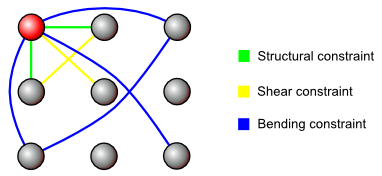
\includegraphics[width=\textwidth]{report/figures/spring_types.png}
    }
    \label{fig:spring_types}
\end{figure}

\paragraph{Structural Springs}
The structural springs are the vertical and horizontal connections between the vertices, which ensures that the model stays in one piece.
However, they alone are not enough, as the model can collapse into itself in a two dimensional space\cite{jeff_lander_real_time_cloth} this can be seen in figure~\ref{fig:structural_springs_collapsing}.

\begin{figure}[H]
    \centering
    \caption{Cloth of only structural springs in the process of collapsing into itself}
    \scalebox{0.5}{
    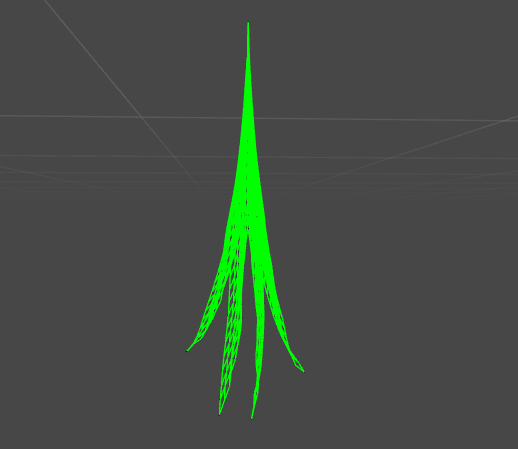
\includegraphics[width=\textwidth]{report/figures/structural_collapse.png}
    }
    \label{fig:structural_springs_collapsing}
\end{figure}

\paragraph{Shear Springs}
Shear springs fixes the issue mentioned above by connecting each vertex to their diagonal neighbours.
When the vertices are about to start collapsing in on themselves the shear springs will push them apart again\cite{jeff_lander_real_time_cloth}.
With this the model also acts in a more three dimensional space, as the vertices needs to make use of the third dimension to satisfy the shear springs, as seen in figure~\ref{fig:shear_springs_collapsing}.
\begin{figure}[H]
    \centering
    \caption{Cloth of structural and shear springs, preventing it from collapsing into 2D space}
    \scalebox{0.5}{
    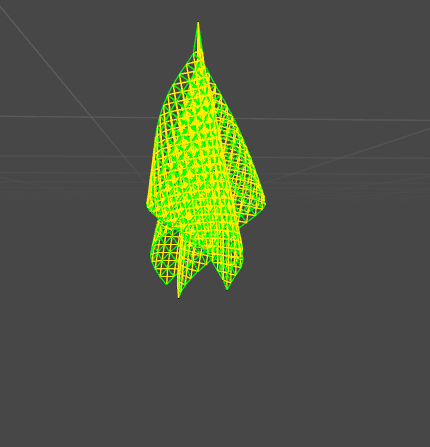
\includegraphics[width=\textwidth]{report/figures/shear_collapse.png}
    }
    \label{fig:shear_springs_collapsing}
\end{figure}

\paragraph{Bending Springs}
Technically you only need these structural and shear springs to create an ok looking cloth simulation,
however a third type of spring called bending springs can be added.
These are connected between each vertex and their second neighbour,
which can help fix cases where the second neighbour of a vertex is unrealistically placed in the system.
This in general leads to the cloth becoming more flat, as extreme differences between the vertices are corrected for
through the second neighbouring vertices\cite{jeff_lander_real_time_cloth}.
While not as obvious, this can be seen in figure~\ref{fig:bending_springs_collapsing}.
\begin{figure}[H]
    \centering
    \caption{Cloth of structural, shear, and bending strings, preventing it from bending unrealistically into itself.}
    \scalebox{0.5}{
    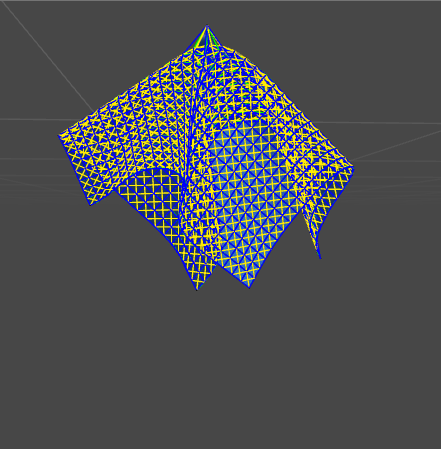
\includegraphics[width=\textwidth]{report/figures/bending_collapse.png}
    }
    \label{fig:bending_springs_collapsing}
\end{figure}

\todo{Mention that all the springs have the same force, that might be something we want to change}

% This might be what is creating wrinkles?
% Double check that this is actually the case.
% Without
%
% 1 -- 2
%      |
%      3
% With
% ------------|
% 1 -- 2 ---| |
%           3 -

\subsubsection{Implementation}
In this implementation we keep all the springs within a collection, each spring knowing which two vertices they are connected to and the desired rest length of the spring.
Upon update we iterate through all the vertices and calculate their new positions based on the Verlet integration scheme.
Following the update is fixing the constraints. This is done by iterating through all the springs and correcting the distance between the vertices it is connected to.
This needs to be done several times as to avoid the model seeming to elastic.
The code for this can be seen in listing~\ref{code:satisfy_constraints}.


\begin{figure}
\begin{lstlisting}[label={code:satisfy_constraints},language=csharp,caption={Semi-Implicit Euler Integration}]
private void FixedUpdate()
{
    for (int step = 0; step < ConstraintIterations; step++)
    {
        for (int i = 0; i < mSprings.Count; i++)
        {
            var spring = mSprings[i];
            var diff = mPositions[spring.V2Idx] - mPositions[spring.V1Idx];
            var dist = diff.magnitude;
            var correction = (diff * (1 - spring.RestDistance / dist)) * 0.5f;

            mPositions[spring.V1Idx] += correction;
            mPositions[spring.V2Idx] -= correction;
        }
    }
}
\end{lstlisting}
\end{figure}

\subsubsection{Usage}
Due to its more sophisticated nature this implementation offers more flexibility than the previous one.
Simulation of entire pieces of clothes like curtains or flags are obvious ways of using this model.
However, it is not a requirement of the model that every vertex in a mesh are simulated and part of the mass spring system, you can also just simulate parts of it.
An example here is if you have a character wearing a dress, you probably do not need that every part of the dress
has realistic cloth physics, it is probably enough that just the bottom of the dress reacts to the environment
to create a believable appearance.

Another use case with this model could be to have cloth that tears at a certain point because it is stretched too much,
or that parts of the cloth is cut off. This should not be too difficult, you would need to remove the springs between
the vertices that have been disconnected from the rest of the model.
Additionally, you would have to ensure that all the cuts were in line with the triangles of the mesh.

\subsubsection{Issues}
Although there are many advantages of this model, like how it is relatively easy to implement, gives quite good results and cannot "explode", it does suffer from a few issues.
A problem with this implementation is that it can get into unsolvable states.
I.e. when you apply forces to model continuously it can get into a situation where it never rests.
Such a situation can be seen in the following video \todo{Add video, and change sentence to: Such a situation can be seen at (point) in the video}.
Here the forces of gravity are continuously being applied to the vertices, in the real world the bottom
of this cloth would stop moving after a while. However, in this implementation the cloth never stops moving
because the springs never manage to get into a situation where they all are "satisfied".
This is a weakness of the kinematic approach which was chosen for this implementation\cite{math_for_games}.

The number of times you need to iterate over the constraints to satisfy them is also an issue.
Too few iterations and the cloth will look too elastic, too many iterations and it can seem too hard,
additionally, the more iterations you add, the more processing time is needed, which can become a performance problem.

\subsubsection{Extensions}
Matthew Fisher\cite{matthew_fisher} suggests some extensions to the model,
such as quilting. Currently the cloth looks like infinitely thin silk, which is not particularly realistic,
quilting would add thickness to the model, allowing it to look and act more like wool or cotton. 
Fisher suggests doing this with a marching cubes algorithm.
However, that would potentially be more costly to simulate and to draw.
Another extension could be self collision or collision with other soft bodies, however, this is very challenging to implement
and quickly ends up being really expensive in terms of performance as well.
Moving these calculations to the GPU is also a possibility, as a lot of the calculations are data parallel and would probably benefit quite a lot for being executed in a parallel environment.
This implementation does not make any distinction between the different types of springs, extending the implementation to react differently based on the different spring types could lead to more realistic behavior.

\todo{Bring up how an extension is to do this on a gpu}

\todo{Should I also look into the Catlike Coding water deformation thingy, as it is another way of doing mesh deformation}


\todo{The technology ahead, ask if this could be used with tesselation and be done on the GPU?}
\todo{Discuss how mass spring damper model also used for other stuff, such as water simulation. Look at Just Cause water implementation article on gamasutra}
